%!TEX root = ../template.tex
%%%%%%%%%%%%%%%%%%%%%%%%%%%%%%%%%%%%%%%%%%%%%%%%%%%%%%%%%%%%%%%%%%%%
%% chapter3.tex
%% NOVA thesis document file
%%
%% Chapter with lots of dummy text
%%%%%%%%%%%%%%%%%%%%%%%%%%%%%%%%%%%%%%%%%%%%%%%%%%%%%%%%%%%%%%%%%%%%

\typeout{NT FILE chapter3.tex}%
\label{cha:neurobehav}

% (fold)
\newcommandx{\obs}[2][1=]{\todo[linecolor=lightgray,backgroundcolor=lightgray,bordercolor=white,#1]{#2}}
\NewDocumentCommand{\dummyref}{m}{\textcolor{red}{#1}}
% (end)

\chapter{Non-linear mixed representations improve behavioral readouts} 
% Decoding behavior from Purkinje-cells suggests non linear (...) 

\pagebreak

\section{Abstract}


%%%%%%%%%%%%%%%%%%%%%%%%%%%%%%%%%%%%%%%%%%%%%%%%%%%%%%%%%%%%%%%%%%%%%%%%%%%%%%%
%%                                                                           %%
%%                           INTRODUCTION                                    %%
%%                                                                           %%
%%%%%%%%%%%%%%%%%%%%%%%%%%%%%%%%%%%%%%%%%%%%%%%%%%%%%%%%%%%%%%%%%%%%%%%%%%%%%%%
\section{Introduction}


\begin{compactitem}
    \scriptsize
    \item Purkinje cells are required for coordination
    \item Purkinje cell simple spike rate encodes kinematics and position
    \item Population providing readouts (DCN convergence + Shadmehr)
    \item Recent mixed selectivity proposes efficient encoding schema
\end{compactitem}

\vspace{10pt}

Based on histological and circuit characterization studies, the cerebellum is proposed to be a key structure involved in learning. Within this framework, Purkinje cells are regarded as the primary computational units of the cerebellum.
\obs{This should be in chapter 1 (intro)}
During locomotion, the timing of strides across all limbs must be precise to maintain stability, and any motor errors, whether internal or external, must be flexibly compensated for. Internal errors are defined as those arising from motor noise, while external errors refer to unexpected changes in the environment \cite{wolpert_internal_1995}.

Cerebellar lesions are known to result in movement ataxia, where the ability of humans or animals to produce well-timed, coordinated movements is impaired. This loss of function in the cerebellum aligns with the expectation that the motor system can no longer estimate the sensorimotor consequences of motor commands \cite{bastian_cerebellar_1996, bastian_learning_2006, machado_quantitative_2015}. Specifically, localized perturbation of Purkinje cells that project to a single cerebellar nucleus abolishes the learning of a locomotor paradigm without entirely compromising the animals' ability to walk \cite{darmohray_spatial_2019}. This and similar findings support the notion of Purkinje cells as the cerebellum's computational units, suggesting that they must process and encode limb-related signals (\dummyref{refs on Purkinje cell transient perturbation}). 

% \textbf{This raises the question of what signals Purkinje cells receive and integrate to achieve coordination between multiple limbs.}
% \textbf{This raises the question of whether and how Purkinje cells combine signals from multiple limbs achieve coordination between multiple limbs.}
\textbf{This raises the question of whether and how limbs may be represented in Purkinje cells.}

Early Purkinje cell recordings during locomotion have demonstrated that Purkinje cell simple spike rates are modulated during the stride cycle in cats, and are sensitive to position and velocity in rats and mice \cite{udoSimpleComplexSpike1981, armstrongDischargesPurkinjeCells1984, smithSensorimotorcorrelatedDischargeRecorded1995, sauerbreiStructuredVariabilityPurkinje2015}).
\obs{missing some mouse refs}
In non-human primates, Purkinje cell firing has been recorded during single arm reaching tasks, revealing responses to preferred directions, velocities, or combinations of both \cite{coltzCerebellarPurkinjeCell1999}.
By recording multiple neurons separately, it has been shown that Purkinje cells exhibit a variety of neural responses. Their tuning functions can be associated with different locomotor events, phase-shifts, and even contain more than one oscillation per locomotor cycle \cite{sarnaikControlVoluntaryOptogenetically2018, muzzuEncodingLocomotionKinematics2018}.


% There is, however, a knowledge gap in cerebellar encodin

% \begin{tcolorbox}[title=Definition: Non-linear responses]
%     Any non-monotonic response to a parameter, i.e., not accurately described by a straight line (\textcolor{red}{Coltz Ebner 1999 Monkey})
% \end{tcolorbox}

Moreover, a single DCN neuron receives input from hundreds to thousands of Purkinje cells \cite{personSynchronyNeuralCoding2012}. Given the convergence of Purkinje cells to nucleus neurons, one expects the DCN to perform some sort of readout from Purkinje cell populations. 

\textbf{Under what conditions could this readout be used for coordination?}

Recent computational work has proposed the concept of \textit{mixed selectivity}. Neurons often contain representations of multiple features across a repertoire of behavioral tasks, yielding unclear single neuron tuning functions and high dimensional representations even at the level of single cells. The framework of mixed selectivity proposes that this might be an effective mechanism for efficient readouts of single variables from neural populations by downstream brain structures \cite{rigottiImportanceMixedSelectivity2013}. 
Moreover, it's possible that a degree of non-linearity highlights specific combinations of task variables \cite{johnstonNonlinearMixedSelectivity2020}.

In this chapter, I describe a neural decoder approach for studying how non-linear interactions between limbs may be useful for downstream readouts.

%%                                                                           %%
%%%%%%%%%%%%%%%%%%%%%%%%%%%%%%%%%%%%%%%%%%%%%%%%%%%%%%%%%%%%%%%%%%%%%%%%%%%%%%%




%%%%%%%%%%%%%%%%%%%%%%%%%%%%%%%%%%%%%%%%%%%%%%%%%%%%%%%%%%%%%%%%%%%%%%%%%%%%%%%
%%                                                                           %%
%%                           METHODS AND RESULTS                             %%
%%                                                                           %%
%%%%%%%%%%%%%%%%%%%%%%%%%%%%%%%%%%%%%%%%%%%%%%%%%%%%%%%%%%%%%%%%%%%%%%%%%%%%%%%

\section{Methods and Results}

\subsection{Encoder: simulating a pseudo-population of Purkinje cells during common behavior}

Ramirez, Marques et al.~conducted cell-attached patch clamp voltage recordings of individual Purkinje cells in the right cerebellar hemisphere during head-fixed mouse locomotion on a wheel. In this task, mice ran on a freely moving wheel and locomotor behavior was recorded for offline paw tracking.

\begin{figure}[h]
    \centering
    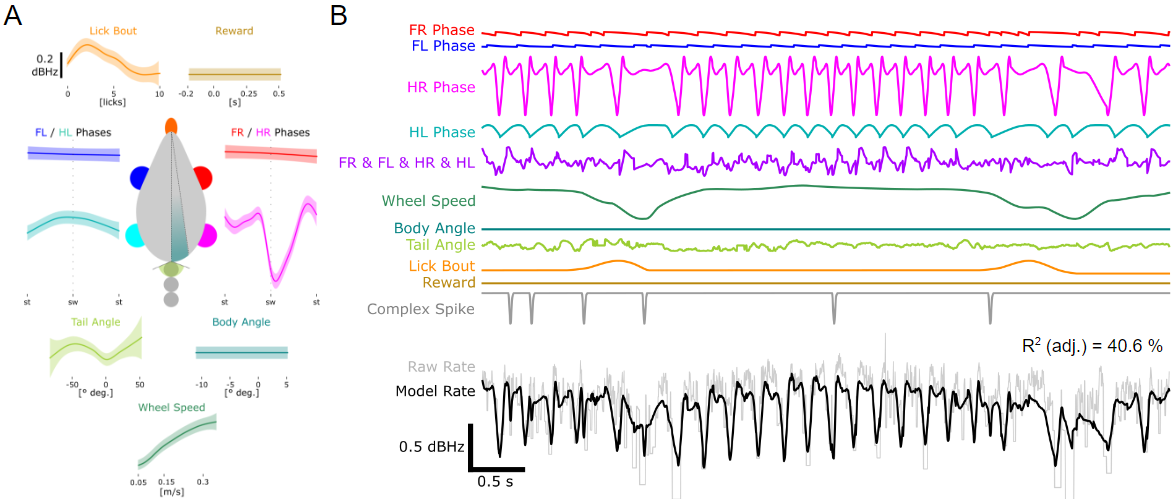
\includegraphics[width=0.99\linewidth]{Chapters/Figures/chapter3/gam-methods.png}
    \caption{Purkinje cells are modulated by multiple limbs. \textbf{A} Stride phases are extracted from positions for each paw by linearly interpolating between swing and stance events.}
    \label{fig:gam-methods}
\end{figure}
\obs{Figure needs to be updated. B) should go out, A should become C, and A should be about preproc}

Generalized additive models (GAMs) were used to infer tuning functions of each neuron to the different paws by decomposing firing rates into additive components modulated by each limb. Tuning functions were specified in a phase space defined between stance onset events for each paw. \textbf{Results show that most Purkinje cells are tuned to more than one limb, and some neurons are modulated by non-linear combinations of limb phases}\cite{ramirezburitica2024nonlinear}.

Since the cerebellum is implicated in whole-body coordination, it is no surprise than multilimb representations arise in single Purkinje cells. Signals from multiple limbs should be integrated at some point in the circuit to achieve precise coordination. However, at the level of single Purkinje cells, it is hard to isolate single limb kinematics. We asked whether populations of Purkinje cells might employ an encoding mechanism akin to non-linear mixed selectivity to facilitate downstream kinematic readout by the DCN, something we presume would be useful in the context of coordination and locomotor learning.

To test whether non-linear mixed selectivity would be useful in this context, we evaluated multiple kinematic readouts from Purkinje cell population firing. However, since each session yielded recordings for one neuron, we simulated firing rates for a pseudo-population during an example behavior segment. The firing rate of each neuron was defined as:
\begin{gather}
\label{eq:fr-paws}
\text{Simulated FR} = r_0 + \sum_{p=1}^{4} r_{p} + r_{NLI}
\intertext{\indent Where:}
  \begin{tabular}{l c l}
    \(r_{0}\)       & : & baseline firing rate  \\
    \(r_{p}\)       & : & firing rate component due to paw \(p\) \\
    \(r_{NLI}\)     & : & firing rate component due to non-linear interaction between paw phases \\
  \end{tabular}\nonumber
\end{gather}

\(r_{0}\), \(r_{p}\) and \(r_{NLI}\) were estimated from the GAMs. Firing rates were estimated by applying the tuning function of each neuron to the paw phases during the example behavior segment (encoding), as depicted in \ref{fig:encdec}A.

\begin{tcolorbox}
Encoding: simulate firing rates from kinematics
\end{tcolorbox}

\begin{figure}[h!]
    \centering
    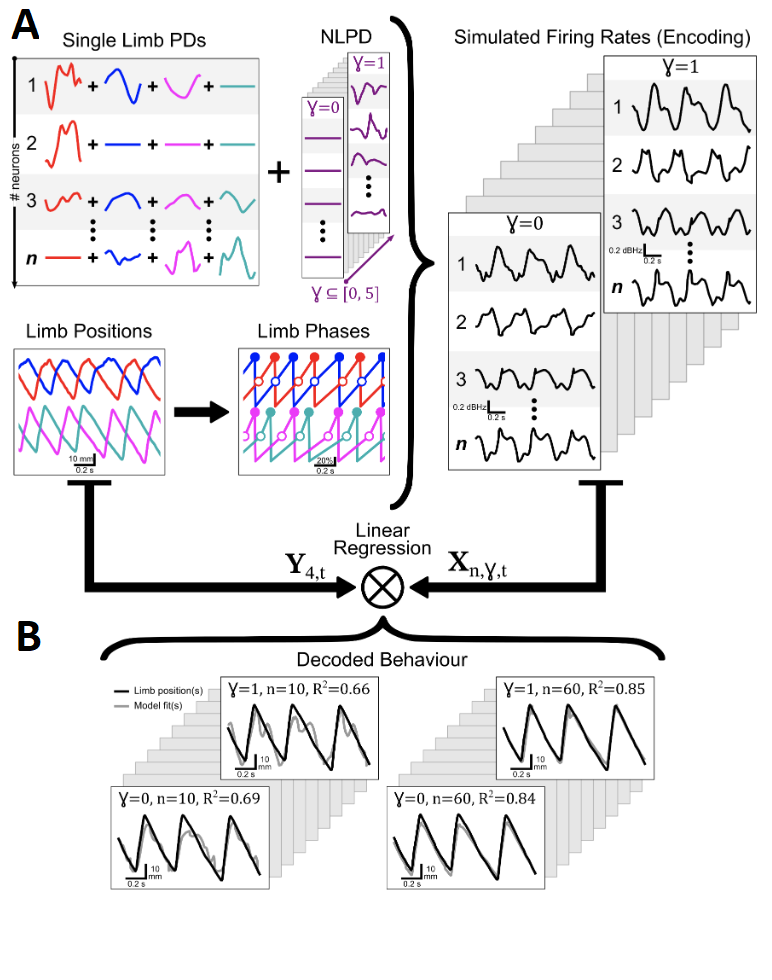
\includegraphics[width=.6\linewidth]{Chapters//Figures//chapter3/encoderdecoder.png}
    \caption{Enter Caption}
    \label{fig:encdec}
\end{figure}


\subsection{Decoder: recovering paw positions and readout metrics}



\subsection{Non-linearly mixed neural representations of multiple limbs improve kinematic decoding from pseudo-populations of Purkinje cells}.

\begin{figure}[h]
    \centering
    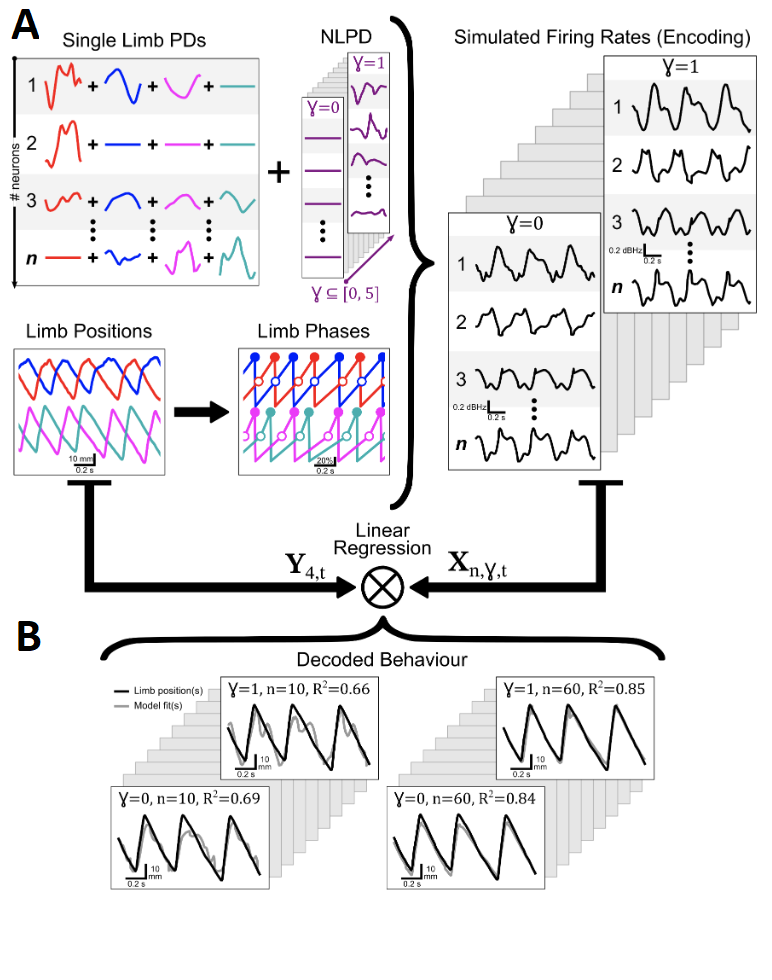
\includegraphics[width=1\linewidth]{Chapters//Figures//chapter3/encoderdecoder.png}
    \caption{Enter Caption}
    \label{fig:encdecccc}
\end{figure}


%%%%%%%%%%%%%%%%%%%%%%%%%%%%%%%%%%%%%%%%%%%%%%%%%%%%%%%%%%%%%%%%%%%%%%%%%%%%%%%
%%                                                                           %%
%%                           DISCUSSION                                      %%
%%                                                                           %%
%%%%%%%%%%%%%%%%%%%%%%%%%%%%%%%%%%%%%%%%%%%%%%%%%%%%%%%%%%%%%%%%%%%%%%%%%%%%%%%

\section{Discussion}

%%%%%%%%%%%%%%%%%%%%%%%%%%%%%%%%%%%%%%%%%%%%%%%%%%%%%%%%%%%%%%%%%%%%%%%%%%%%%%%
%%                                                                           %%
%%                           METHODS SUPP                                    %%
%%                                                                           %%
%%%%%%%%%%%%%%%%%%%%%%%%%%%%%%%%%%%%%%%%%%%%%%%%%%%%%%%%%%%%%%%%%%%%%%%%%%%%%%%
\section{Methods supplement}
% \subsection{Animal model: wildtype mice}
% \subsection{Behavioral paradigm}
% \subsection{GAM analysis}
% 

in bouts of 30 seconds. After this period, a mechanical brake would engage the wheel forcing the animal to stop for \textbf{\textcolor{red}{X}} seconds. Water rewards were given after \textbf{\textcolor{red}{Y}} meters of locomotion. Paw positions were estimated via markerless tracking on videos acquired at 330 fps from a combination of bottom view mirror and side positioned camera.

Under this framework limb phases are extracted from limb positions by linearly interpolating 2 segments corresponding to swing and stance periods. The continuous phase for each paw is then binned into multiple basis functions (Figure \ref{fig:gam-methods}A).

% \section{Purkinje cells encode multiple limbs}

Mice move in a coordinated manner where diagonal limb pairs move together. When using traditional approaches such as event rasters, the resulting tuning functions are similar between two pairs of limbs (Figure \ref{fig:behavioral-correlations}).
\obs{this should be made explicit in the introduction and here should be just a slight reminder}

\par This aspect of locomotion poses a difficulty when isolating paw contributions to firing rate. Two correlated limbs will have similar tuning functions, and they will be in anti-phase relative to the homolateral pair.

% \subsection{GAMs decompose firing rate into limb tuning}

Each basis function serves as a regressor in a generalized additive model (GAM). Organizing continuous variables into temporal basis sets allows decorrelating the contributions of highly correlated limb signals which would otherwise suffer from statistical instability \cite{ramirezburitica2024nonlinear}.
GAMs take the following form:

\begin{gather}
\label{eq:gam-eq}
\text{Firing Rate} = \beta_0 + \sum_{i=1}^{N} \sum_{j=1}^{M} \beta_{i,j} \cdot \phi_{i,j} + \epsilon
\intertext{\indent Where:}
  \begin{tabular}{l c l}
    \(\beta_0\)     & : & \(y\) intercept  \\
    \(N\)           & : & number of behavioral regressors \\
    \(M\)           & : & number of bins / basis functions \\
     \(\phi_{i,j}\) & : & basis function for behavioral regression \(i\) bin \(j\) \\
    \(\beta_{i,j}\) & : & model coefficient for behavioral regression \(i\) bin \(j\) \\
    \(\epsilon\)    & : & residuals
  \end{tabular}\nonumber
\end{gather}

and a tuning function is the smoothed collection of \(\beta\) for all \(j\) (\ref{fig:gam-methods}B).

The outputs of the GAM are the coefficients organized in the phase space of each variable, i.e., partial dependency functions (PDPs), that can be interpreted as tuning functions (Figure \ref{fig:gam-methods}C), as well as the predicted firing rate.


% ...........................................



Ramirez et al.~fitted one GAM per recorded Purkinje cell

% \subsection{Emergence of a non-linear component for limb mixing in Purkinje cells}

GAMs also allow specifying non-linear interactions between regressors under the hypothesis that some variance in the firing rate is due to specific combinations of features. In our case, these combinations would occur in a 4 dimensional phase space combined from all paws.
\par 





% \section{Neural decoding}
% Describe the concepts behind neural decoding here, mostly from Glaser and Kording.
% \subsection{Encoding: building pseudo-population firing rates from single-cell recording sessions}
% \subsection{Decoding: statistical metrics for behavioral readouts}
% \subsection{Purkinje cell non-linear mixed representations improve behavioral readouts}
